%!TEX root = ../report.tex

\documentclass[../report.tex]{subfiles}
\begin{document}

We begin by discussing The Firefighter Problem and explain how it can be adapted to a rudimentary model of disease; we then discuss Percolation Theory and its use in a graph-theoretic context; we end by discussing compartmental graph models of disease, in particular examining the differential equations required to describe such models exactly.

\subsection{The Firefighter Problem}

The Firefighter Problem, which we refer to as simply {\scshape Firefighter}, was first introduced by Hartnell \cite{hartnell_1995} and models an outbreak of fire with a firefighter strategically blocking its path. {\scshape Firefighter} has been the primary foundation for our approaches to modelling over the last year.

We formalise {\scshape Firefighter} as follows: at $t=0$, a fire breaks out at some vertex $v_0$ of graph $G$. The firefighter then `protects' another vertex\footnote{\,This has been extended to $n$ vertices in some research, but here we wish to illustrate for simplicity the original single-vertex outbreak form of the problem.} of $G$. A protected vertex is protected for the remainder of the game; it is inflammable \textit{ad infinitum.} Similarly, a vertex that has been on fire is `burnt' for the rest of the game and cannot ignite again. The fire spreads to any immediate neighbouring vertices that are neither protected nor burnt. Then, the firefighter may protect another vertex, the fire spreads again and so on. 
%The following is a decision formulation given by Finbow and MacGillivray for {\scshape Firefighter} on a tree \cite{finbow_2009}:
%\vspace{1mm}
%
%\begin{center}
%\noindent\fbox{%
%	\centering\parbox{0.8\linewidth}{%
%{\scshape Firefighter}\\ \indent
%{\scshape Instance:} A rooted graph $(G,r)$ and an integer $k\geq 1$.\\ \indent
%{\scshape Question:} Is there a finite sequence $d_1, d_2,\dots d_t$ of vertices of the graph $G$ such that:
%	\begin{enumerate}[label=\roman*]
%		\item $d_i$ {is neither burned nor defended at time} $i$,
%		\item {At time} $t$, no undefended vertex is adjacent to a burning vertex, and
%		\item {At least} $k$ {vertices are saved at the end of time} $t$?
%	\end{enumerate}
%	}%
%}%
%\end{center}

Common questions to ask in {\scshape Firefighter} include: how do we minimise the number of vertices that will be burnt? In a given class of trees, what is the average number of burnt vertices? Is the problem NP-complete?

If we let each vertex be an individual and let the edges between them represent social contact. This is a simple model for disease infection, which is where our interest in the game enters. There are many natural contextualisations of {\scshape Firefighter} beyond modelling disease spread, which we may choose to apply our work to in future - for instance, we may think of edges representing virtual contact between individuals on social media, yielding a model for the spread of viral internet memes \cite{obrien_2019}.

\subsection{Percolation Theory}
\label{sec:perc}

Widely known and used in physics, statistics and mathematics, Percolation theory involves modelling scenarios as $n$-dimensional graphs, so application to {\scshape Firefighter} is not entirely unexpected. Hence, we will now examine percolation theory in order to later explain the utility we have found it may yield in extending and expanding modelling work from {\scshape Firefighter}.

In percolation, the edges between vertices in the graph can be either `open' or `closed' with probability $p$ and $1-p$ respectively. We can think of percolation problems as liquid being poured onto a porous material and whether there is a path from hole to hole along open paths through the material. Note that removing more and more edges moves us towards a critical point at which removing further edges would cause the graph to fall apart into smaller clusters of vertices and edges that have no access to each other \cite{grimmett_1999}. This is known as `bond' percolation, as edges correspond to bonds in many of its applications.
\begin{figure}[ht]
	\centering
		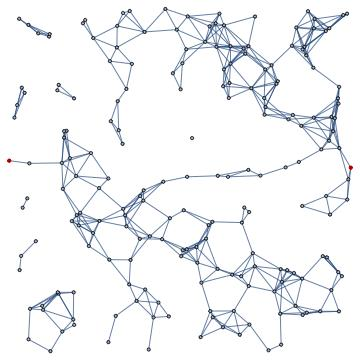
\includegraphics[width=0.45\linewidth]{percolated-graph.jpg}
	\caption{A graph that has been subject to percolation.}
	\label{fig:percolated-graph}
\end{figure}

Several authors have suggested percolation as a possible approach to {\scshape Firefighter} \cite{finbow_2009}. In this context, we could determine the critical point to see how we might contain the fire to a smaller cluster that cannot spread to the wider graph. For {\scshape Firefighter}, site percolation is more applicable: rather than considering open or closed \emph{edges} (`bonds') between vertices as in bond percolation, we consider each \emph{vertex} (`site') as being `occupied' or `unoccupied' with probability $p$ and $1-p$ respectively.

Formally, we consider a point lattice $\mathbb{L}$ and denote the open cluster as $C(x)\text{,~where~}x\in\mathbb{L}$ is the local origin of the cluster. This cluster $C(x)$ is defined as the set of all vertices that can be reached from open paths beginning at the nucleation site, $x$. Then, we are particularly interested in the \emph{percolation probability}:
$$
\theta(p) = \mathbb{P}_p(\,|C(0)|=\infty\,),
$$
and the \emph{critical probability} (or \emph{percolation threshold}):
$$
p_c = \sup\{\,p \mid \theta(p)=0\,\}.
$$
Here, $\mathbb{P}_p$ is the product measure given by:
$$
\displaystyle \mathbb{P}_p=\prod_{v\in\mathbb{L}^d}\mu_v
$$
where $\mu_v$ is the \emph{Bernoulli measure}, which returns $p$ when $v$ is open and $1-p$ when $v$ is closed \cite[p. 28]{klenke_2014}. Analytically, others have shown that in the case of a two-dimensional regular point lattice, the critical probability is $p_c=1/2$ \cite{kersten_1980}.

%%%%%%%%%%

\subsection{Markovian SIR epidemics on networks}

In the past year, we have also spent significant time understanding, applying and expanding results around equations describing Markovian $SIR$ graph models of disease exactly \cite{kiss_2014} so we will now provide a review of the key work in this area and its utility. We will go on to detail the work done so far in extending the results from this paper in the following section.

In \cite{kiss_2014}, the authors note that there are generally three approaches to compartmental models of disease. We can:
\begin{enumerate}
	\item Take averages at population level, 
	\item Maintain a probabilistic view by considering the full state space, or
	\item Begin modelling at the level of vertices and build up to larger structures from there.
\end{enumerate}

The second of the three approaches has been the focus of much of our work, as will be seen in the following section. The latter of these three approaches is the one used in the work on Markovian SIR graph epidemics being discussed currently: begin by considering equations for single vertices, then consider dependencies on pairs, then triples and so on until we reach the full system size. Such equations are well defined and consistent, which is not difficult to see.

The work presented has two aims. Firstly, to provide an exact, deterministic representations of Markovian $SIR$ epidemics on graphs with and without loops. Secondly, to identify a link between the structural properties of the graphs and the viability of closures that can be used to write down exact systems of equations that can be numerically evaluated. In particular, the authors show this structural link is founded on cut-vertices and bridges. Cut-vertices are vertices that, if removed from a connected graph, result in the formation of two (or more) disconnected sub-graphs. Bridges are edges that lie between two cut-vertices.

The authors spend significant time expanding intuitions on the identification of closures, which allow us to approximate or even exactly specify higher-order moments in terms of lower-order moments. They claim this is well known to be feasible for tree-like graphs and for graphs with loops starting from some specific initial conditions. They present some examples to develop the intuition that ``loops cannot be closed by breaking them down to their component parts."

The main result of the work reveals an important relation between structure of the graph used in the epidemic model and types of closures that are feasible using cut-vertices and bridges.

They also prove an impressively general result: if a graph with $N$ vertices and  $E$ edges has $T$ triangles and no larger loops than size 3 (meaning also that triangles cannot have overlapping edges), an upper bound on the size of the system of equations describing the system dynamics can be calculated:
$$
2N + 3E + 7T \leq 10N
$$

The authors also provide a ``recipe-like" approach to establish the feasibility of writing down an exact representation for a given graph even more generally. They use this to provide an upper bound for the number of equations required to describe epidemic dynamics exactly:
$$
\displaystyle N_{EQ}(G)=\sum^P_{i=1}m_if_i - 2\sum^{L}_{j=1}(\text{Ind}(v_{i_j})-1).
$$
where $P$ is the number of distinct sub-graphs produced when the original graph is spliced into independent sub-graphs through cut-vertices, $m_i$ represents the number of equations required to describe the corresponding sub-graph $i$, $f_i$ is the frequency or count of the sub-graph $G_i$ and $\text{Ind}(v_{i_j})$ is the number of sub-graphs to which the cut-vertex $v_{i_j}$ belongs.

This takes a sum across the number of equations for all sub-graphs and adjusts to account for unnecessary multiplications caused by cut-vertices being part of multiple sub-graphs, which is a move made in illustrative examples throughout the work.

\end{document}